\section{Introduction}
\subsection{Background}
\subsubsection{Stewart Platform}
\subparagraph*{Description of Mechanism}
\paragraph{}A stewart platform is a platform with six degrees of freedom (DOF). The six-degrees-of-motion platform is capable of moving in three linear directions and
three angular directions singly or in any combination.
It comprises a triangular/rectangular/circular plane called the platform, of which each of the corners (for triangualar platform in this case) is connected through a three-axis joint to one of three legs. This is shown in Fig.1.1.
\begin{figure}[!h]
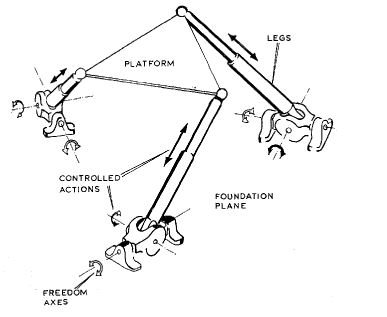
\includegraphics{Figures/Fig1}
\caption{General arrangement}
\end{figure}
\paragraph{}Each leg is connected to the ground by a two-axis joint where: One of these axes is
normal to the leg and is provided with a means for control wheareas, the other axis is normal to the first and is not provided with a means for control.
Each leg also has controllable means for extending its length. These control means include:
\begin{enumerate}
\item Use of two hydraulic jacks
\item Screw Jacks
\item Rotary actuator
\item Levers
\item Linear co-ordinate control
\item Strength
\end{enumerate}
\paragraph{}These shall be discussed in detail at a later stage.

\subparagraph{Application}
\paragraph{}The six DOF Stewart Platform provides an elegant design for simulating flight conditions which finds applications in the safe training of pilots. The mechanism differs from other simulators in that it has no fixed axes relative to the ground, and therefore within the limits of amplitude of the design it can truly simulate the conditions of banking by carrying the simulation of control surfaces into the axes of the new attitude.

\subsubsection{Force Balance}
\subsection{Problem statement}
(Insert your content)
\subsection{Objectives}
(Insert your content)
\subsection{Justification of the study}
\paragraph{}Additive manufacturing offers the ability to produce intricate products and parts with lower development costs, shorter lead times, less energy consumed during manufacturing as well as less material waste. This method can be used to manufacture delicate components such as the bipolar plates with elimination of the risks involved such as breakage of brittle Graphene material during production.     
\paragraph{}Precise control of reactant flow and pressure, stack temperature, and membrane humidity will increase the fuel cell’s robustness as well as efficiency.
\paragraph{}The goal of this research is to develop physic-based dynamic models of fuel cell systems and fuel processor systems and then apply multivariable control techniques to study their behavior. The analysis will give insight into the control design limitations and provide guidelines for the necessary controller structure and system re-design.
